\documentclass{article} % For LaTeX2e
\usepackage{nips14submit_e,times}
\usepackage{amsmath}
\usepackage{amsthm}
\usepackage{amssymb}
\usepackage{mathtools}
\usepackage{hyperref}
\usepackage{url}
\usepackage{algorithm}
\usepackage[noend]{algpseudocode}
%\documentstyle[nips14submit_09,times,art10]{article} % For LaTeX 2.09

\usepackage{graphicx}
\usepackage{caption}
\usepackage{subcaption}

\def\eQb#1\eQe{\begin{eqnarray*}#1\end{eqnarray*}}
\def\eQnb#1\eQne{\begin{eqnarray}#1\end{eqnarray}}
\providecommand{\e}[1]{\ensuremath{\times 10^{#1}}}
\providecommand{\pb}[0]{\pagebreak}
\DeclarePairedDelimiter\ceil{\lceil}{\rceil}
\DeclarePairedDelimiter\floor{\lfloor}{\rfloor}

\newcommand{\E}{\mathrm{E}}
\newcommand{\Var}{\mathrm{Var}}
\newcommand{\Cov}{\mathrm{Cov}}

\def\Qb#1\Qe{\begin{question}#1\end{question}}
\def\Sb#1\Se{\begin{solution}#1\end{solution}}

\newenvironment{claim}[1]{\par\noindent\underline{Claim:}\space#1}{}
\newtheoremstyle{quest}{\topsep}{\topsep}{}{}{\bfseries}{}{ }{\thmname{#1}\thmnote{ #3}.}
\theoremstyle{quest}
\newtheorem*{definition}{Definition}
\newtheorem*{theorem}{Theorem}
\newtheorem*{lemma}{Lemma}
\newtheorem*{question}{Question}
\newtheorem*{preposition}{Preposition}
\newtheorem*{exercise}{Exercise}
\newtheorem*{challengeproblem}{Challenge Problem}
\newtheorem*{solution}{Solution}
\newtheorem*{remark}{Remark}
\usepackage{verbatimbox}
\usepackage{listings}
\usepackage{mathrsfs}
\title{ProbLimI: \\
Problem Set I}


\author{
Youngduck Choi \\
CIMS \\
New York University\\
\texttt{yc1104@nyu.edu} \\
}


% The \author macro works with any number of authors. There are two commands
% used to separate the names and addresses of multiple authors: \And and \AND.
%
% Using \And between authors leaves it to \LaTeX{} to determine where to break
% the lines. Using \AND forces a linebreak at that point. So, if \LaTeX{}
% puts 3 of 4 authors names on the first line, and the last on the second
% line, try using \AND instead of \And before the third author name.

\newcommand{\fix}{\marginpar{FIX}}
\newcommand{\new}{\marginpar{NEW}}

\nipsfinalcopy % Uncomment for camera-ready version

\begin{document}


\maketitle

\begin{abstract}
This work contains solutions to the exercises of the problem set I. The
chosen problems are 1,2, and 4.
\end{abstract}

\bigskip

\begin{question}[1]
\hfill
\begin{figure}[h!]
  \centering
    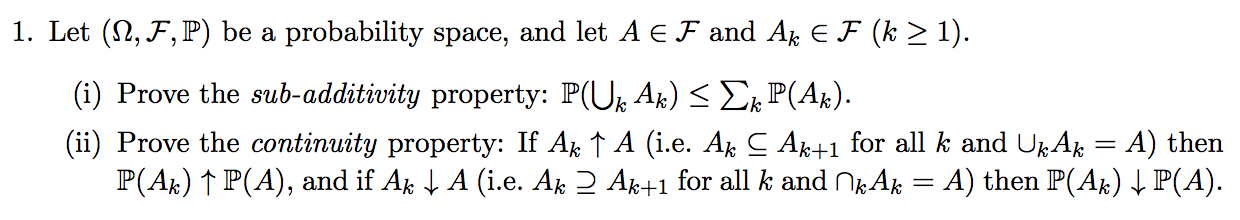
\includegraphics[width=0.7\textwidth]{problim-e1-p1.png}
\end{figure}
\end{question}
\begin{solution} \hfill \\
\textbf{(i)} Note that we have finite additivity property of measure, 
as the emptyset belong to any $\sigma$-field by definition.
We first have 
\eQb
A,B \in \mathscr{F}, A \subset B \implies \mathbb{P}(A) \leq \mathbb{P}(B) 
\>\>\> (*),
\eQe
because
\eQb
\mathbb{P}(B) &=& \mathbb{P}((B \setminus A) \cup A) = \mathbb{P}(B \setminus A)
+ \mathbb{P}(A).
\eQe
Now, define $A_0 = \emptyset$, and 
\eQb
\tilde{A}_k &=& A_k \setminus (\bigcup_{0 \leq n < k} A_n) \>\>\> (k \geq 1).
\eQe
It follows that $\{ \tilde{A}_k \}$ is a pairwise disjoint collection such that
\eQb
\bigcup_k \tilde{A}_k = \bigcup_k A_k \>\>\> \text{and}  \>\>\>
\tilde{A}_k \subset A_k \>\>\> (k \geq 1).
\eQe
The union equality holds, since
if $x \in \bigcup_k A_k$, then $x \in A_{k'}$
for some $k'$, and  $x \in \tilde{A}_{k^*}$ , where 
\eQb
k^* = \inf\{k ; x \in A_k \}, 
\eQe
as $x \notin A_k$ for $k < k^*$ and $x \in A_{k^*}$. 
Hence, by countable additivity, 
\eQb
\mathbb{P}(\bigcup_k A_k) = \mathbb{P}(\bigcup_k \tilde{A}_k ) 
= \sum_k \mathbb{P}(\tilde{A}_k) \leq \sum_k \mathbb{P}(A_k),
\eQe
where the last inequality follows from $(*)$. \hfill $\qed$

\newpage

\textbf{(ii)} Define $A_0, \tilde{A}_0 = \emptyset$ and 
\eQb
\tilde{A}_k &=& A_k \setminus A_{k-1} \>\>\>\> (k \geq 1). 
\eQe  
By finite additivity and the fact that 
$\{A_k\}$ is increasing, we have, for any $k \geq 1$,
\eQb
\mathbb{P}(A_k) &=& \mathbb{P}(A_{k-1} \cup (A_{k} \setminus A_{k-1})) 
= \mathbb{P}(A_{k-1}) + \mathbb{P}( A_k \setminus A_{k-1}), \\ 
\eQe
and by re-arranging 
\eQb
\mathbb{P}(\tilde{A}_k) &=& \mathbb{P}(A_k) - \mathbb{P}(A_{k-1}). \\ 
\eQe
Now, $\{ \tilde{A}_k \}$ are disjoint, so by countable additivity, we have
\eQb
\mathbb{P}(A) = 
\mathbb{P}(\bigcup_{k} A_k) &=& \mathbb{P}(\bigcup_{k} \tilde{A}_k) 
= \sum_{k} \mathbb{P}(\tilde{A}_k) = \lim_{k \to \infty} \sum_{n = 1}^{k} 
\mathbb{P}(A_n) - \mathbb{P}(A_{n-1}) \\
&=& \lim_{k \to \infty} \mathbb{P}(A_k) - \mathbb{P}(A_0) = \lim_{k \to \infty}
\mathbb{P}(A_k),
\eQe
as required. Now, we show the continuity from above. Note that $\{A_k^c\}$
forms an increasing collection.
By the DeMorgan's law, and continuity from below,
\eQb
1 - \mathbb{P}(\bigcap_k A_k) &=& \mathbb{P}((\bigcap_k A_k)^c) 
= \mathbb{P}(\bigcup_k A_k^c) = \lim_{k\to \infty} \mathbb{P}(A_k^c) 
= 1 - \lim_{k \to \infty} \mathbb{P}(A_k), 
\eQe 
so 
\eQb
\mathbb{P}(A) &=& \mathbb{P}(\bigcap_k A_k) =  \lim_{k \to \infty} \mathbb{P}(A_k), 
\eQe
as required. \hfill $\qed$


\end{solution}

\newpage

\begin{question}[2]
\hfill
\begin{figure}[h!]
  \centering
    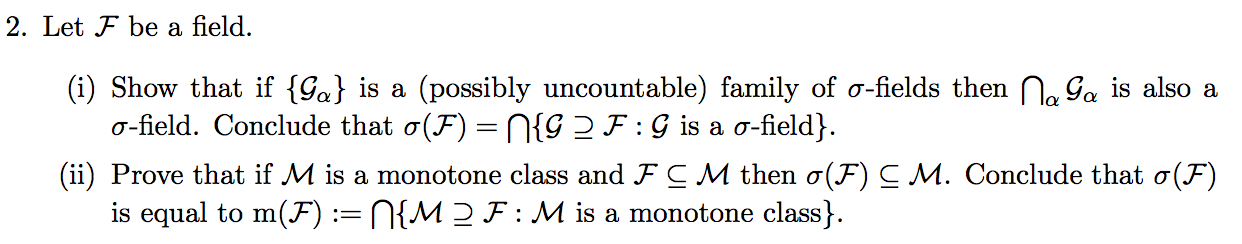
\includegraphics[width=0.7\textwidth]{problim-e1-p2.png}
\end{figure}
\end{question}
\begin{solution} \hfill \\
\textbf{(i)}
We just note that the index set must be non-empty.
As $\emptyset$ and $\Omega$ are in $\mathscr{G}_{\alpha}$ for all $\alpha$,
by the $\sigma -$field property of each $\mathscr{G}_{\alpha}$, 
it follows that $\emptyset, \Omega \in \bigcap_{\alpha}
\mathscr{G}_{\alpha}$. Now, it suffices to show
that
\eQb
A \in \bigcap_{\alpha} \mathscr{G}_{\alpha} &\implies& 
A^c \in \bigcap_{\alpha} \mathscr{G}_{\alpha}, 
\\
\{ A_n\} \subset \bigcap_{\alpha} \mathscr{G}_{\alpha}  &\implies& 
\bigcap_n A_n \in \bigcap_{\alpha} \mathscr{G}_{\alpha}.
\eQe
If $A \in \bigcap_{\alpha} \mathscr{G}_{\alpha}$ then, $A \in \mathscr{G}_{\alpha}$
for all $\alpha$, and by the $\sigma -$field assumption on each $\mathscr{G}_{\alpha}$,
it follows that $A^c \in \mathscr{G}_{\alpha}$ for all $\alpha$, so $A^c \in
\bigcap_{\alpha} \mathscr{G}_{\alpha}$. \\ 

\smallskip

If $\{A_n \} \subset \bigcap_{\alpha} \mathscr{G}_{\alpha}$, then $\{ A_n \} \subset
\mathscr{G}_{\alpha}$ for all $\alpha$, and by the $\sigma -$ field assumption on
each $\mathscr{G}_{\alpha}$, it follows that $\bigcap_n A_n \in \mathscr{G}_{\alpha}$
for all $\alpha$, so $\bigcap_n A_n \in \bigcap_{\alpha} \mathscr{G}_{\alpha}$. 

\smallskip

First, note that $\{\mathscr{F} \subset \mathscr{G} \>\> | \>\>
\mathscr{G} \>\> \text{is a } \> \sigma \text{-field} \}$ 
is non-empty, as $2^{\Omega}$ 
belongs to it. So by the above result $
\mathscr{G}^* = \bigcap \{ \mathscr{F} \subset \mathscr{G} \>\> | \>\> 
\mathscr{G} \>\> \text{is a } \> \sigma \text{-field} \}$ is a $\sigma$-field,
and we see that $\mathscr{F} \subset \mathscr{G}^*$. So far, we have shown that
there exists a $\sigma$-field that contains $\mathscr{F}$. 
From construction, it is trivial that for any $\sigma$-field such that 
$\mathscr{F} \subset  \mathscr{G}$, we have
\eQb
\mathscr{G}^* \subset \mathscr{G}
\eQe
so this shows that there exists a smallest $\sigma$-field that contains
$\mathscr{F}$. The uniqueness follows as well, because if $\mathscr{G}_1$
and $\mathscr{G}_1$ are both smallest $\sigma$-field, then by definition
\eQb
\mathscr{G}_1 \subset \mathscr{G}_2 \>\> \text{and} \>\> \mathscr{G}_2
\subset \mathscr{G}_1,
\eQe
so
\eQb
\mathscr{G}_1 = \mathscr{G}_2.
\eQe
Hence, we have shown precisely that for $\mathscr{F}$ (obviously the proof will go
through for any collection), there exists a unique $\sigma$-algebra that 
contains $\mathscr{F}$ and 
notationally  
\eQb
\sigma(\mathscr{F}) &=& 
\mathscr{G}^* = 
\{ \mathscr{F} \subset \mathscr{G} : \mathscr{G} \> 
\text{ is a } \sigma-\text{field} \},
\eQe 
as required. \hfill $\qed$ 

\bigskip

\textbf{(ii)} We first establish that as above the intersection of
a collection montone classes $\{ \mathscr{M}_{\alpha} 
\}$ is a montone class. It suffices to 
show that 
\eQb
\{ A_{n}\} \subset \bigcap_{\alpha} \mathscr{M}_{\alpha} \>\>
\text{ and } \>\> A_n \subset A_{n+1} \>\> \forall n \geq 1 
&\implies& \bigcup_{n} A_n \in \bigcap_{\alpha} \mathscr{M}_{\alpha},  
\eQe
which holds, because by montone class property of each $\mathscr{M}_{\alpha}$,
$\bigcup_{n} A_n \in \mathscr{M}_{\alpha}$ for each $\alpha$, so 
$\bigcup_{n} A_n \in \bigcap_{\alpha} \mathscr{M}_{\alpha}$. Now, 
as above $2^{\Omega}$ is a monotone class, we deduce that there exists
a unique smallest monotone class containing any subset of $2^{\Omega}$, which 
we call the generated montone class.  

\bigskip
Given that $\mathscr{F}$ is a field, we contend that the montone class generated by 
$\mathscr{F}$, $m(\mathscr{F})$ is a $\sigma$-field. Then, by definition of the 
generated $\sigma$-field, we would get the desired conclusion that $\sigma(\mathscr{F})
\subset \mathscr{M}$ for any $\mathscr{M}$ that contains $\mathscr{F}$, because 
\eQb
\sigma(\mathscr{F}) \subset m(\mathscr{F}) \subset \mathscr{M}.
\eQe
It suffices to show that 
\eQb
m(\mathscr{F}) \>\> \text{ is a field },
\eQe
since for $\{ A_n\} \subset m(\mathscr{F})$, we have
\eQb
\bigcup_{n} A_n &=& \bigcup_{n} \bigcup_{k=1}^{n} A_n \in m(\mathscr{F}),
\eQe
where the last inclusion holds by the field, and monotone class property of 
$m(\mathscr{F})$. As $X \in \mathscr{F} \subset m(\mathscr{F})$, it again suffices to
show
\eQb
A,B \in m(\mathscr{F}) &\implies& A\setminus B , A\cap B \in m(\mathscr{F}).
\eQe
Fix $A \in m(\mathscr{F})$, and consider 
\eQb
m(A) &=& \{B \in m(\mathscr{F}) \> ;\> A\setminus B , B \setminus A, 
A \cap B  \in m(\mathscr{F}) \}.
\eQe 
One should note that $m(A)$ is a monotone class and
\eQb
A \in m(B) &\iff& B \in m(A) \>\> (*),
\eQe
by the symmetry in the definition.
It suffices to show that  $m(\mathscr{F}) \subset m(A)$. First, we prove the
case when $A \in \mathscr{F}$. Then, by definition of field, it follows that
\eQb
A \subset m(A) \>\> \text{ and } m(\mathscr{F}) \subset m(A), 
\eQe 
where the last set inclusion holds as $m(A)$ is a monotone class. Now,
we extend to the case when $A \in m(\mathscr{F})$. By the above result and
the $(*)$ equivalence,
\eQb
A \in m(B) \>\> \text{and} \>\> B \in m(A),
\eQe
for any $B \in \mathscr{F}$. Hence, it follows that
\eQb
\mathscr{F} \subset m(A) \>\> \text{and} \>\> m(\mathscr{F}) \subset m(A), 
\eQe
and we are done. \hfill $\qed$

\bigskip

For sake of completeness, we use the above statement to conclude the remaining
statement. From the statement, 
it follows that, for any monotone class $\mathscr{M}$ such that
$\mathscr{F} \subset \mathscr{M}$, 
\eQb
\sigma(\mathscr{F}) &\subset& \mathscr{M},
\eQe
so
\eQb
\sigma(\mathscr{F}) &\subset& 
\bigcap\{\mathscr{F} \subset \mathscr{M} :
\mathscr{M} \> \text{ is a monotone class} \} = m(\mathscr{F}). 
\eQe 
Conversely, as a $\sigma$-field is a monotone class, we have that
\eQb
m(\mathscr{F}) &=& 
\bigcap\{\mathscr{F} \subset \mathscr{M} :
\mathscr{M} \> \text{ is a monotone class} \} 
\subset 
\bigcap \{\mathscr{F} \subset \mathscr{G} :
\mathscr{G} \> \text{ is a } \sigma-\text{field} \} =  
\sigma(\mathscr{F}), \\ 
\eQe
so
\eQb
\sigma(\mathscr{F}) &=& m(\mathscr{F}),
\eQe
as required. In passing, we mention that the intersection of any family
of monotone class is a monotone class and the proven result is known
as the monotone class lemma. \hfill $\qed$

\end{solution}

\newpage

\begin{question}[3]
\hfill
\begin{figure}[h!]
  \centering
    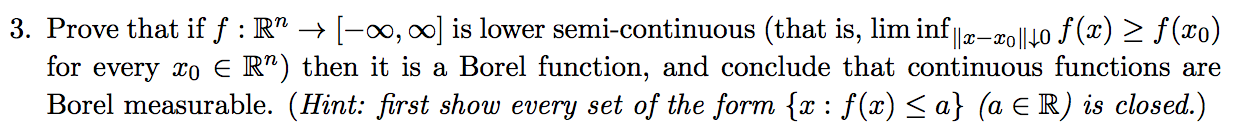
\includegraphics[width=0.7\textwidth]{problim-e1-p3.png}
\end{figure}
\end{question}
\begin{solution} \hfill \\
We first establish an important observation follows: 
Let $X,Y$ be topological spaces,
and $\mathscr{B}_X$, $\mathscr{B}_Y$ are respective Borel $\sigma$-fields. Then,
for any $f: X \to Y$, 
\eQb
f \text{ is continuous } &\implies& f \text{ is } (B_X,B_Y) \text{ measurable}.
\eQe
This holds, because open sets are generators of any Borel $\sigma$-field, and
by continuity, we obtain that the generators of the image are mapped to
the $\sigma$-field on the domain. This problem gives a stronger result of this nature
in this concrete setting, where the domain is $\mathbb{R}^n$ and the image is $[-\infty,
\infty]$, because it shows that the lower semi-continuity is sufficient for 
measurability. In summary, the conclusion holds, as continuity implies
lower continuity, which by the stated result implies measurability.
 
\bigskip
Now, we proceed with the proof. It suffices to show that 
\eQb
A = \{ x \in \mathbb{R}^n : \> f(x) \leq \alpha \},
\eQe
is closed for any $a \in \mathbb{R}$, because closed sets 
belong to the Borel $\sigma$-field, and $\{[-\infty,a]\}_{a}$ form a generator 
of the image $\sigma$-field. We claim that $A$ is closed. Suppose that
$x \in \mathbb{R}^n$ such that there exists $x_n$ from $A$ that $x_n \to x$.
As $||x_n - x|| \to 0$, by the lower-semicontinuity, we obtain
\eQb
f(x) \leq \liminf f(x_n) \leq a ,
\eQe 
so $x \in A$. Hence, $A$ is closed and we are done. \hfill $\qed$
\end{solution}

\newpage 

\begin{question}[4]
\hfill
\begin{figure}[h!]
  \centering
    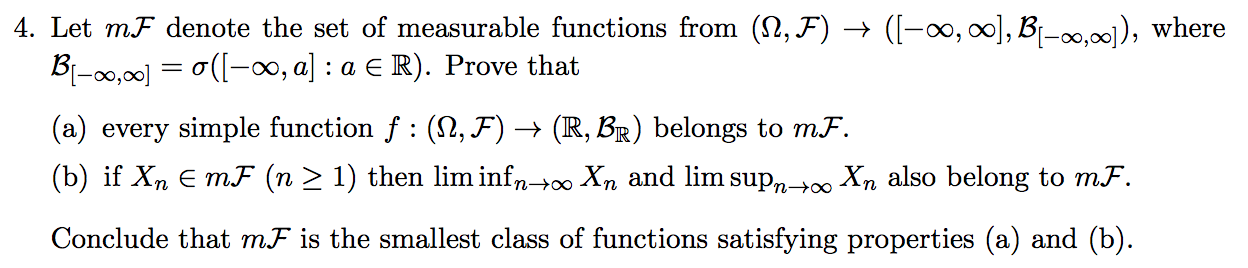
\includegraphics[width=0.7\textwidth]{problim-e1-p4.png}
\end{figure}
\end{question}
\begin{solution} \hfill \\
\textbf{(a)} Let $f$ be a simple function, i.e. 
\eQb
f &=& \sum_{i=1}^{n} a_i X_{E_i},
\eQe
where $a_i \in \mathbb{R}$, $E_i \in \mathscr{F}$ pairwise disjoint
for $1 \leq i \leq n$, and $\bigcup_{i=1}^{n} E_i = \Omega$.
For sake of completeness, we show that $f$ is $(\mathscr{F},\mathscr{B}_{\mathbb{R}})$
measurable. For any $a \in \mathbb{R}$, observe that $f^{-1}((-\infty,a])$ 
is a union of sub-collection (allowing the empty collection) of $\{ E_i \}$, so
it is in $\mathscr{F}$. As it is sufficient to check the measurability condition on
the generators, we conclude that any simple function is $(\mathscr{F},
\mathscr{B}_{\mathbb{R}})$ measurable.

\bigskip

Fix $a \in \mathbb{R}$. 
As $f^{-1}(-\infty) = \emptyset$ and 
$f$ is $(\mathscr{F},\mathscr{B}_{\mathbb{R}})$ measurable, it follows that 
\eQb
f^{-1}([-\infty,a]) &=& f^{-1}(-\infty) \cup f^{-1}((-\infty,a]) \in \mathscr{F}.
\eQe
So, $f$ is $(\mathscr{F}, \mathscr{B}_{\mathbb{[-\infty,\infty]}})$ measurable,
i.e. $f \in m\mathscr{F}$. \hfill $\qed$

\bigskip

\textbf{(b)} Observe that 
\eQb
\liminf_{n \to \infty} X_n &=& \sup_k \inf_{n \geq k} X_n\\
\limsup_{n \to \infty} X_n &=& \inf_k \sup_{n \geq k} X_n\\.
\eQe
Hence, combined with the fact that $\inf_n X_n = -\sup_n - X_n$, 
it suffices to show that $\sup_n X_n$ is measurable.


Fix $a \in \mathbb{R}$. Then, we have
\eQb
(\sup_n X_n)^{-1}([-\infty,a]) &=& \bigcap_n X_n^{-1} ([-\infty,a]) \in \mathscr{F}.
\>\> (*)
\eQe 
We now prove $(*)$. If $w \in \bigcap_n X_n^{-1}([-\infty,a])$, then 
$X_n(w) \in [-\infty,a]$ for all $n$, so $\sup_n X_n(w) \in [-\infty,a]$,
and $w \in \sup_n X_n^{-1} ([-\infty,a])$. If $w \in \sup_n X_n^{-1}([-\infty,a])$,
then $\sup_n X_n(w) \in [-\infty,a]$, which implies $X_n(w) \in [-\infty,a]$ 
for all $n$. Hence, $(*)$ is true and $\sup X_n \in m\mathscr{F}$. 

\bigskip

Let $\mathscr{G}$ be a class of functions such that $(a)$ and $(b)$ are true. 
We wish to show that $m\mathscr{F} \subset \mathscr{G}$. By $(a)$, we know that
simple functions are in $\mathscr{G}$. Now, if $f \in m\mathscr{F}$, then
by the simple approximation lemma, there exists a sequence of simple functions
$\{X_n \}$ such that $X_n$ converges pointwise to $f$. Then, by $(b)$,
\eQb
f = \limsup_{n \to \infty} X_n \in \mathscr{G},
\eQe 
so $m\mathscr{F} \subset \mathscr{G}$, and $m\mathscr{F}$ is the smallest class
of functions satisfying properties $(a)$ and $(b)$. \hfill $\qed$

\end{solution}
\newpage

\end{document}
